\section{The local speedometer of current space}
\label{sec:velocity-geometry}

At a fixed current and speed, the set of instantaneous current velocities is
\[
 \boxed{\gls{sym:vset}=\vect f(\vect i)+\matr B(\vect i)\gls{sym:uset}.}
 \tag{26.1}
\]
It lives in the tangent space attached to the present current point.  Shape
records dynamic anisotropy, displacement of its centre records electrical
drift, and its principal axes identify directions that can be changed quickly
or slowly.  It is a local speedometer, not a static voltage ellipse: the
latter is a set of states satisfying a steady-state voltage inequality,
whereas \(\mathcal V\) is a set of derivatives at one state.

\subsection{Converter sets and their exact images}

For the EESM, an ideal circular stator limit and independent field converter
give the product set
\[
 \mathcal U_{\circ\times I}=
 \{\vect u:u_{\mathrm d}^2+u_{\mathrm q}^2\leq U_{\max}^2,
 |u_{\mathrm f}|\leq U_{\mathrm f,\max}\}.
 \tag{26.2}
\]
It is a cylinder with flat caps, not an ellipsoid.  A quadratic approximation
\[
 \mathcal U_E=\{\vect u:\vect u^{\mathsf T}\matr S^{-1}\vect u\leq1\},
 \quad \matr S=\operatorname{diag}(U_{\max}^2,U_{\max}^2,U_{\mathrm f,\max}^2)
 \tag{26.3}
\]
has a smooth boundary and is convenient for analysis, but couples simultaneous
stator and field utilization more conservatively than the product set.  The
actual two-level inverter hexagon crossed with the field interval maps to a
translated polytope.  All three are legitimate; they answer different
fidelity--cost questions.

For the ellipsoidal approximation, the controlled velocity body has metric
\[
 (\dot{\vect i}-\vect f)^{\mathsf T}\matr G
 (\dot{\vect i}-\vect f)\leq1,
 \qquad
 \boxed{\matr G=\matr B^{-\mathsf T}\matr S^{-1}\matr B^{-1}}.
 \tag{26.4}
\]
In the linear reciprocal model \(\matr B=\matr L^{-1}\), hence
\(\matr G=\matr L^{\mathsf T}\matr S^{-1}\matr L\).  A small eigenvalue of
\(\matr G\) marks a fast direction because a large velocity has unit cost
there.  This reverses the visual intuition from a covariance ellipsoid.

\begin{figure}[tb]
\centering
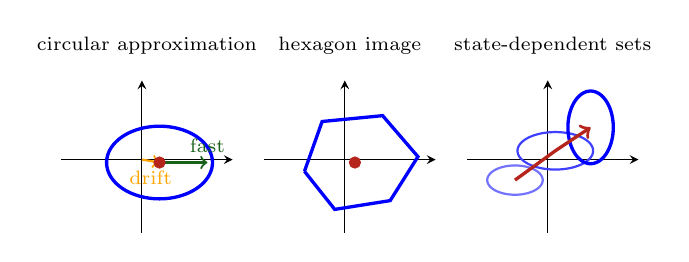
\begin{tikzpicture}[font=\scriptsize]
 \begin{axis}[name=a,width=.31\linewidth,height=.29\linewidth,axis lines=middle,
  xmin=-1.6,xmax=1.8,ymin=-1.25,ymax=1.35,ticks=none,title={circular approximation}]
  \addplot[blue,very thick,domain=0:360,samples=121] ({.35+1.05*cos(x)},{-.05+.62*sin(x)});
  \addplot[only marks,mark=*,BrickRed] coordinates {(.35,-.05)};
  \draw[->,Orange,thick] (axis cs:0,0)--(axis cs:.35,-.05) node[midway,below] {drift};
  \draw[->,ForestGreen!70!black,thick] (axis cs:.35,-.05)--(axis cs:1.3,-.05) node[above] {fast};
 \end{axis}
 \begin{axis}[name=b,at={(a.east)},anchor=west,xshift=4mm,width=.31\linewidth,height=.29\linewidth,
  axis lines=middle,xmin=-1.6,xmax=1.8,ymin=-1.25,ymax=1.35,ticks=none,title={hexagon image}]
  \addplot[blue,very thick] coordinates {(-.8,-.2)(-.2,-.85)(.9,-.7)(1.45,.05)(.75,.75)(-.45,.65)(-.8,-.2)};
  \addplot[only marks,mark=*,BrickRed] coordinates {(.2,-.05)};
 \end{axis}
 \begin{axis}[name=c,at={(b.east)},anchor=west,xshift=4mm,width=.31\linewidth,height=.29\linewidth,
  axis lines=middle,xmin=-1.6,xmax=1.8,ymin=-1.25,ymax=1.35,ticks=none,title={state-dependent sets}]
  \addplot[blue!55,thick,domain=0:360,samples=81] ({-0.65+.55*cos(x)},{-.35+.25*sin(x)});
  \addplot[blue!75,thick,domain=0:360,samples=81] ({.15+.75*cos(x+20)},{.15+.32*sin(x+20)});
  \addplot[blue,very thick,domain=0:360,samples=81] ({.85+.45*cos(x-25)},{.55+.62*sin(x-25)});
  \addplot[BrickRed,very thick,->] coordinates {(-.65,-.35)(.15,.15)(.85,.55)};
 \end{axis}
\end{tikzpicture}
\caption{Local current-velocity sets.  An ellipsoidal converter model gives a
translated ellipse, the exact inverter gives corners, and nonlinear flux or
changing speed moves and deforms the speedometer along a trajectory.}
\label{fig:velocity-sets}
\end{figure}



\subsection{Dynamic whitening}

Choose
\[
 \boxed{\vect z_d=\gls{sym:dwhite}\vect i,
 \qquad \matr D=\matr S^{-1/2}\matr L}
 \tag{26.5}
\]
for a constant linear model.  Then
\[
 \dot{\vect z}_d=-\matr S^{-1/2}\vect r(\vect i,\omega_e)
                 +\matr S^{-1/2}\vect u
             =\vect W(\vect z_d)+\vect v,
 \qquad \|\vect v\|_2\leq1.
 \tag{26.6}
\]
One unit of ellipsoidal voltage authority now produces one unit of controlled
speed in every direction.  The right singular vectors of
\(\matr L^{-1}\matr S^{1/2}\) are the voltage directions, while its left
singular vectors are the fast/medium/slow current directions.  They need not
coincide with either the eigenvectors of the copper-loss matrix or the torque
axes of Section~\ref{sec:whitening}.  Equality requires simultaneous
diagonalizability, a nongeneric commutation condition such as
\([
\matr R,\matr G]=0\).  Static loss whitening answers ``what current is
thermally cheap?''; dynamic whitening answers ``what current derivative is
voltage-cheap?''

For saturation, replace \(\matr L\) by \(\matr L_{\mathrm{diff}}(\vect i)\).
The metric and whitening map then vary with state.  A single global linear
change of coordinates flattens the control body only if the induced metric is
flat and the converter shape is compatible.  Saturation therefore changes the
geometry through which the operating point moves; it is not merely a scalar
parameter perturbation.
